\section{An abstract machine for switches}
\label{s:absmachine}

\begin{figure*}[!t]
  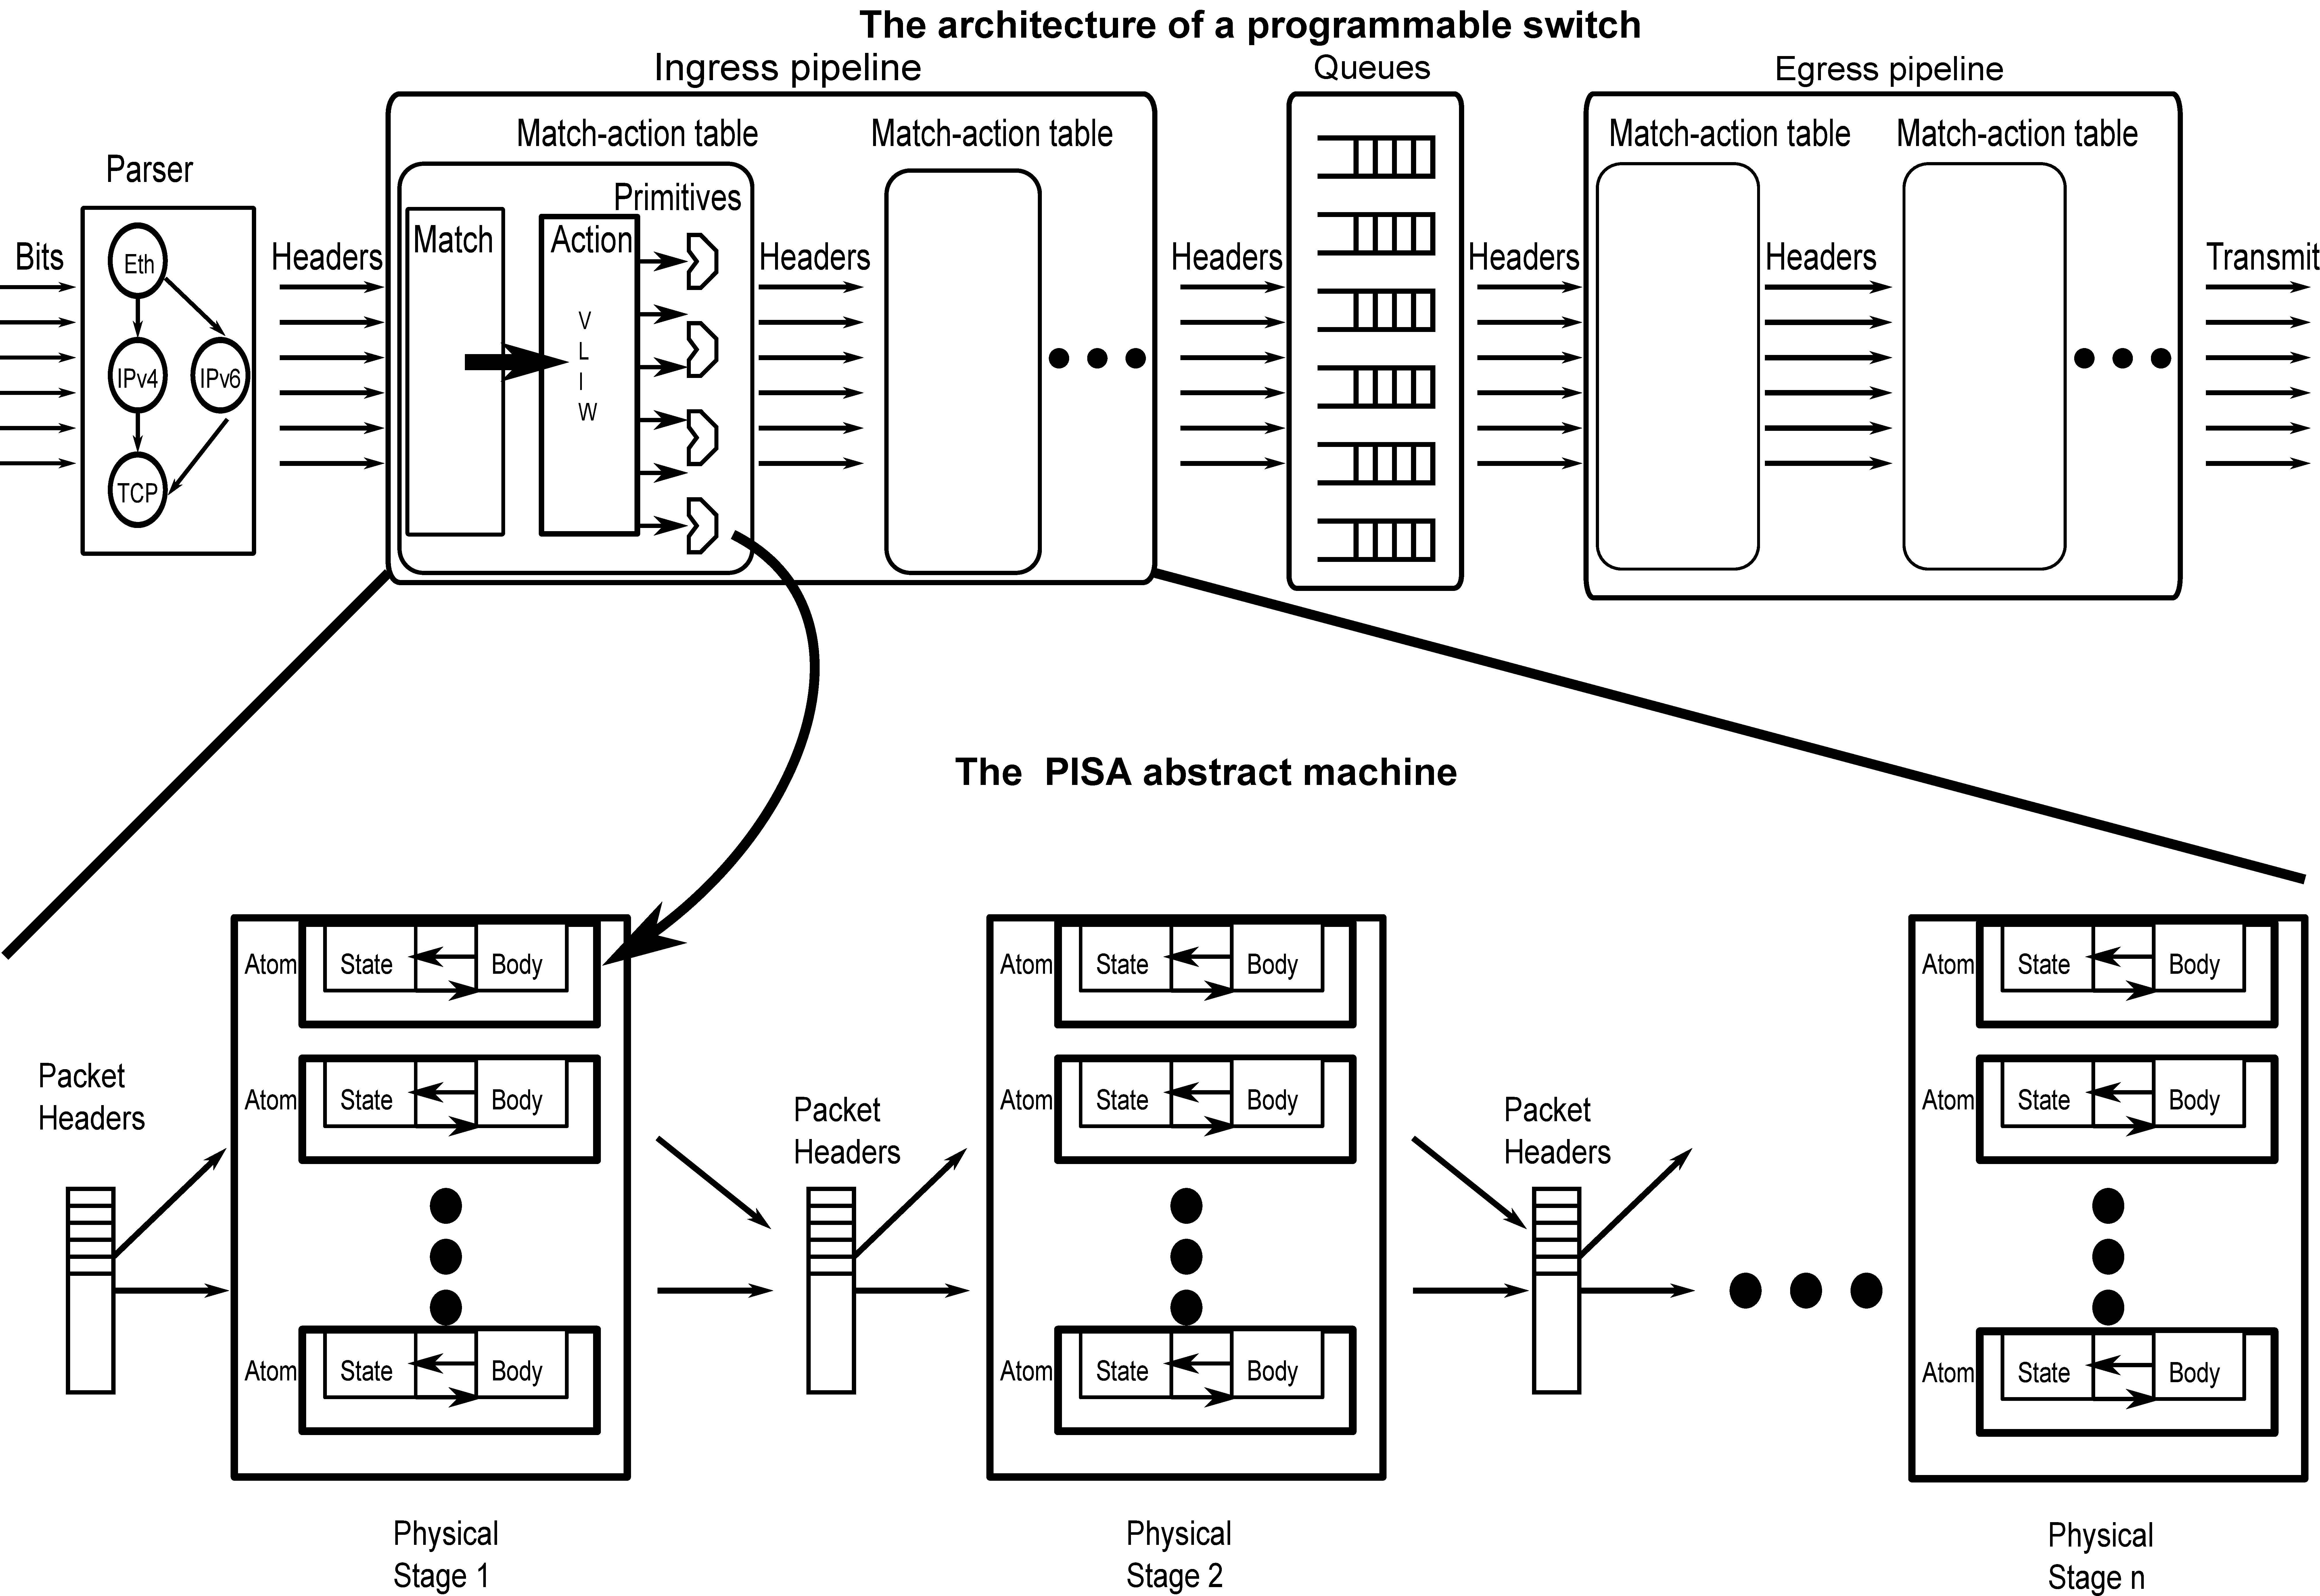
\includegraphics[width=\textwidth]{pisa.pdf}
  \caption{The \absmachine abstract machine and its relationship to
  programmable switch architectures.}
  \label{fig:switch}
\end{figure*}

We first describe \absmachine (Protocol-Independent Switch Architecture~\cite{nick_p4}), 
a family of abstract machines that differ in the functionalities provided 
as discussed below. \absmachine serve as targets for \pktlanguage programs, 
%Here, we go further, by describing an executable machine model that serves as a family
%of compiler targets for \pktlanguage.
the design is inspired by recent programmable switch architectures with
line-rate performance, such as RMT~\cite{rmt}, Intel's
FlexPipe~\cite{flexpipe}, and Cavium's XPliant Packet~\cite{xpliant}. 
These architectures assume the switch model shown at the top of Figure~\ref{fig:switch}.

Packets arriving to the switch are parsed by a programmable parser that turns
packets into header fields. These header fields are first processed by an
ingress pipeline consisting of match-action tables arranged in stages.
Following the ingress pipeline, the packet is queued. Once the packet is
dequeued by the switch scheduler, it is processed by a similar egress pipeline
before being transmitted from the switch. \ac{I am confused. Is what is described
here modeled by \absmachine? Is it just a description of Figure 1?}

\absmachine models a switch pipeline such as the ingress or egress pipeline. A
pipeline consists of a number of pipeline stages that execute synchronously on
every time step. An incoming packet is processed by each stage sequentially until \ac{???}
%Once a pipeline stage
%processes a packet, it hands it off to the next pipeline stage.
Each stage has exactly one time step of latency, where time step is a 
physical quantity determined by the hardware. The inverse of this
time step gives the line rate supported by the pipeline. 

As an abstract machine, \absmachine only models components critical to
data-plane algorithms. In particular, it models the computation that happens in
a match-action table in a stage (i.e., the action half of the match-action
table), but not the match semantics (e.g., direct, ternary, or longest prefix).
\absmachine also does not model packet parsing and assumes that packets
arriving to it are already parsed.\ac{so is pipeline stage a concept in actual
hardware switches or is this something invented in \absmachine? The description 
in two paragraphs earlier seem to imply former, but last paragraph implies the latter.}

\subsection{Atoms: \absmachine's processing units}

In \absmachine, each pipeline stage 
contains a vector of \textit{atoms}. All atoms within the same stage are
run in parallel when the given stage executes.
Informally, an atom is an atomic unit of packet
processing provided natively by a \absmachine machine \ac{you mean hardware? otherwise what
does 'provided natively' mean?} and is represented as a
block of sequential code. An atom completes execution and modifies a packet before
the next packet is processed by that atom. \ac{doesn't 'atomic' already capture this meaning?}
Actions that can be carried out inside an atom include modifying packet headers
and changing the internal state of the switch.
%An atom may also contain internal state that persists across packets and
%influences the atom's behavior from one packet to the next. 
For instance, since \absmachine's instruction set includes loading from and storing to
a state variables, along with arithmetic computation on packet headers, a
switch counter could be written as an atom as follows.\footnote{We use
{\tt p.x} to represent field {\tt x} within a packet {\tt p} and {\tt x} to represent
  the state variable {\tt x} that persists across packets.}
  \begin{lstlisting}[style=customc, numbers=none, frame=none]
  p.tmp   = counter;
  p.tmp2  = p.tmp + 1;
  counter = p.tmp2;
  \end{lstlisting}
Similarly, a stateless operation that sets a packet field (such as P4's
{\tt modify\_field} primitive~\cite{p4spec}) can be written as the atom
below:
\begin{lstlisting}[style=customc, numbers=none, frame=none]
  p.field = value;
\end{lstlisting}

\absmachine generalizes several aspects of existing programmable switch
architectures. The vector of atoms in each stage generalizes RMT's very-large
instruction-word (VLIW)~\cite{rmt} that executes primitive actions on packet
fields in parallel. Internal state within an atom models persistent switch
state such as meters, counters, and P4's register abstraction in a unified
manner. We assume all state is initialized by the switch control plane, which
we don't explicitly model in \absmachine.

\subsection{Constraining atoms}
\label{s:atomConstraints}

\absmachine models a synchronous pipeline where each atom executes on every
time step, reading packet fields at the beginning and writing packet fields at
the end of the time step. All writes happen simultaneously at the end
of a time step; so, \absmachine forbids two atoms in a stage from writing to
the same packet field to remove all data races. \ac{I don't see how writing 
simultaneously at the end of a time step prohibits data races.}

To provide deterministic performance at line rate, atoms must be suitably
constrained.  We impose two such constraints that distinguish \absmachine from
software routers~\cite{click} and network processors~\cite{ixp4xx} that
sacrifice deterministic performance for programmability.

First, \absmachine machines are \textit{shared-nothing}: each atom maintains
certain number of state variables. 
Their values can only be communicated to atoms in
subsequent stages via packet fields. This restriction reflects
the capabilities of line-rate switches: accessing shared memory from multiple
switch stages is technically challenging because it requires multi-ported RAMs
and routing long wires on the chip.

Second, we constrain the complexity of atoms by defining {\it atom templates}
(\S\ref{ss:code_gen}).  Informally, an atom template is a program that is
guaranteed to terminate and specifies how atoms are executed. One example is an
ALU with a restricted set of primitive operations to choose from
(Figure~\ref{fig:alu_in_sketch}). Atom templates allow us to create different
\absmachine machines that support different atoms natively. As programmable
switches evolve, we expect the computational capabilities of atoms to evolve as
well. However, atoms cannot be arbitrarily complex: a programmable switch's
line rate is inversely proportional to the maximum execution latency of all its
atoms. \ac{and we expect such templates be designed by hardware engineers 
and exposed by \absmachine. ?}
